\documentclass[11pt,a4paper]{article}
\usepackage{a4wide}
\usepackage{graphicx}
\usepackage{epsfig}
\usepackage{amsmath}
\usepackage{amsfonts}
\usepackage{amssymb}
\usepackage{ngerman}
\usepackage[utf8]{inputenc}
\usepackage{multirow}
\usepackage{hyperref}
\usepackage{float}
\usepackage{url}
\usepackage{csvsimple}



\begin{document}
\Large\textbf{{{\noindent Übungsblatt 4 - Hochleistungsrechnen\\}}}
\textbf{{Leistungsanalyse\\}}
Tim Kilian, Joscha Fregin, Stefan Knispel


\section{Messung 1}

Bei der Messung 1 wurden die Parameter wie folgt gewählt:
- Threadanzahl ansteigend von 1 bis 12 \\
- Jacobi-Methode \\
- Interlines 512 \\
- Störfunktion 2 \\
- Anzahl an Iterationen \\
- 1100 Iterationen \\
Es wurde auf dem Rechnerknoten west5 gerechnet!
\noindent In der Abbildung \ref{messung1} ist die Berechnungszeit gegen die Anzahl der verwendeten Threads dargestellt. Die Berechnungszeit für einen einzelnen Thread dauert erwartungsgemäß am längsten. Bei zwei verwendeten Threads halbiert sich die Berechnungszeit näherungsweise. 
Plottet man die Berechnungszeit gegenüber der Anzahl der Threads erhält man einen exponentiellen Verlauf. Hier ist deutlich zu erkennen, dass ab einer Verwendung von 6 Threads der Gradient sehr gering ist. Man erhält keine deutliche Verbesserung in der Berechnungszeit mehr im Vergleich zur Anzahl an Threads. 
Bei der Verwendung von 12 Threads verkürzt sich die Berechnungszeit im Vergleich zu der mit einem Thread bei uns um den Faktor 11.5. Damit liegen wir innerhalb des geforderten Bereiches.

\begin{figure}[htb]
\centering
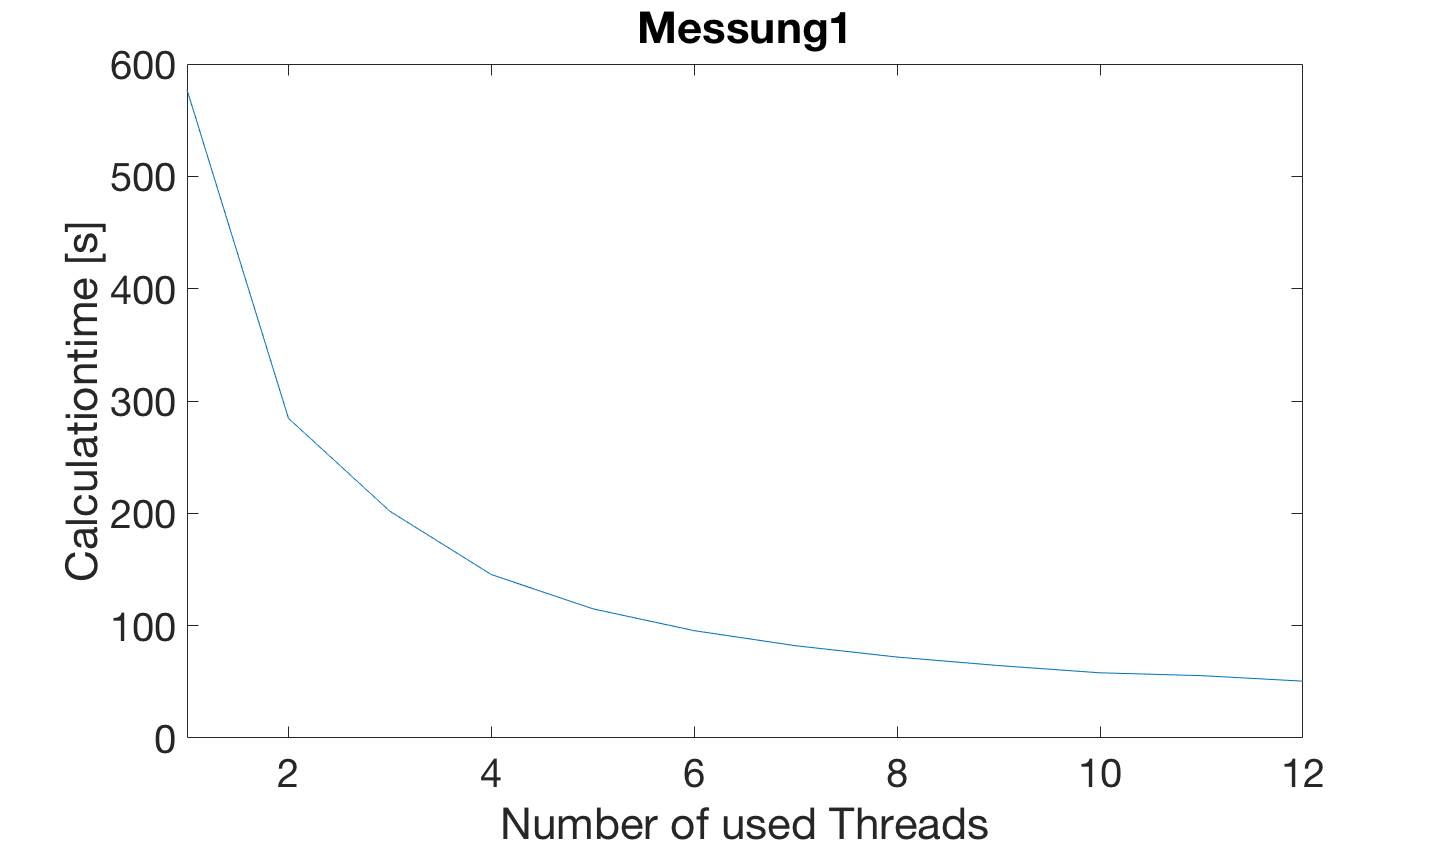
\includegraphics[width=1.0\textwidth,angle=0]{Messung1.png}
\caption{Messung 1 mit 512 Interlines und 1100 Iterationen.}
\label{messung1}
\end{figure}



\section{Messung 2}
Es wurde auf dem Rechnerknoten west5 gerechnet!
In der Abbildung \ref{messung2} ist die Berechnungszeit gegen die Anzahl der Interlines dargestellt. Es ist nicht eindeutig zu erkennen, ob hier ein exponentieller Verlauf vorliegt. Dazu müsste mit noch weiteren Interlines gerechnet werden. Jedoch ist bei einer Anzahl von 1,2 oder 4 Interlines kein Unterschied in der Berechnungszeit zu erkennen. Jeder Durchlauf brachte Berechnungszeiten zwischen 0.3 und 0.9 Sekunden zum Vorschein. Das kommt durch die zu klein gewählte Matrix. Bei einer Zeilenanzahl von maximal 4 kann nicht jeder Thread eine Zeile zum Berechnen übernehmen. Die Berechnungszeit müsste theoretisch zwischen 1 und 12 Interlines fast identisch sein. Ab einer Interlines Anzahl von 13 müsste diese erst wieder ansteigen, da dann mehr Zeilen als Threads vorhanden sind. 

\begin{figure}[htb]
\centering
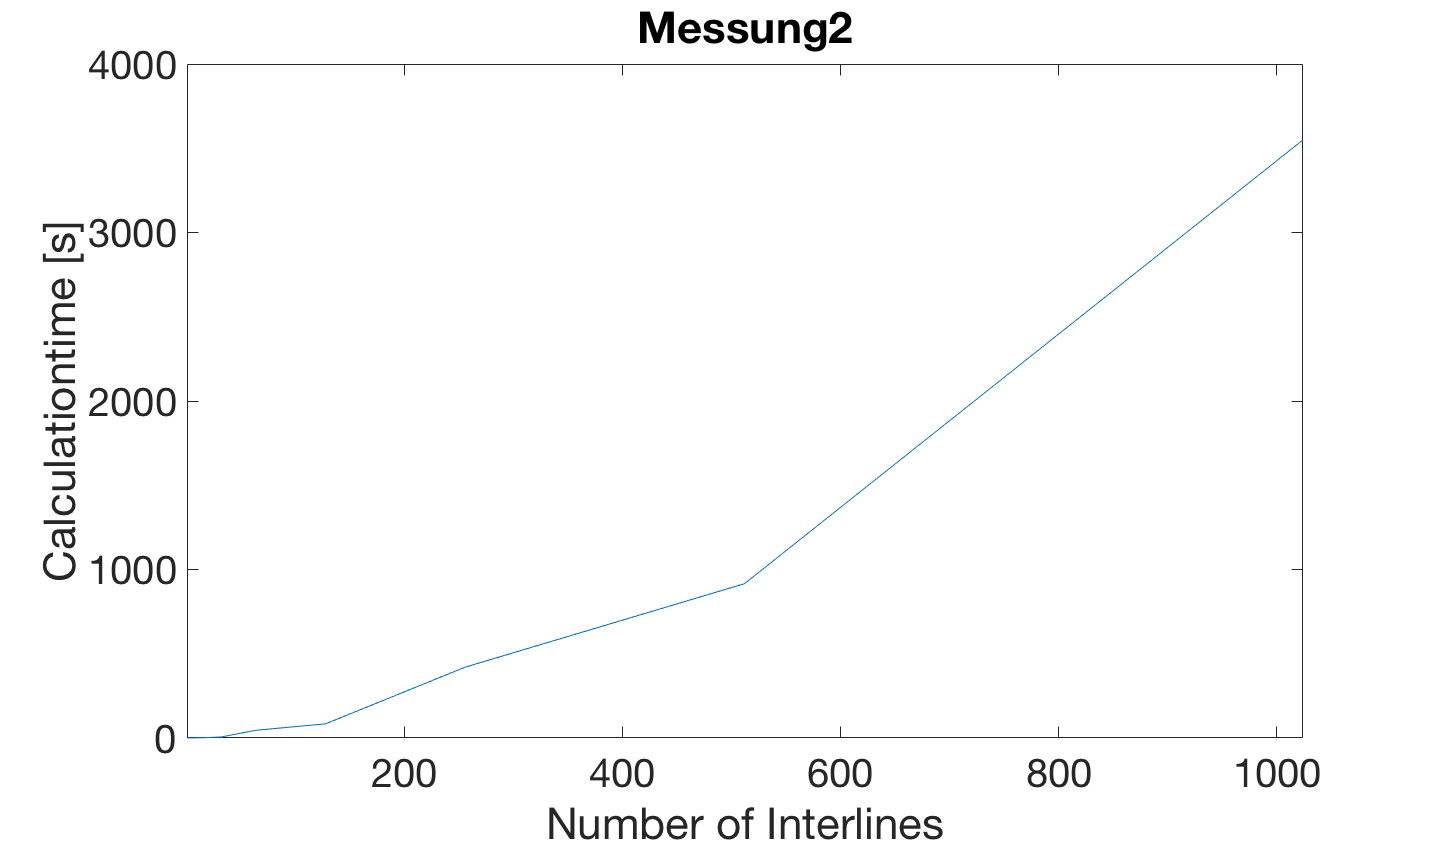
\includegraphics[width=1.0\textwidth,angle=0]{Messung2.png}
\caption{Messung 2 mit 20000 Iterationen und 12 Threads.}
\label{messung2}
\end{figure}



\end{document}
